\section{Testy jednostkowe}
W celu zachowania poprawności działania zostały przygotowane testy mające na celu sprawdzanie działania mappera. Testy opiewały o podstawowe funkcjonalności jak i te bardziej złożone. Za wykonywanie testów odpowiedzialny jest plik \mintinline{php}|tests.php|, zawiera on główną klasę \mintinline{php}|Tests|, która w konstruktorze powołuje konkretne testy rozszerzające klasę \mintinline{php}|Test|. Wszystkie testowane klasy zawierają metodę \mintinline{php}|test()|, w której zawarta jest logika testu. Metoda ta, musi zwrócić wartość wywołania  \mintinline{php}|pass()| - jeżeli test się powiedzie, lub \mintinline{php}|fail()| - jeżeli dojdzie to jakiegoś zdarzenia. Metody te odpowiednio obsłużą raportowanie wyników testu. 

\begin{figure}[ht]
	\centering
	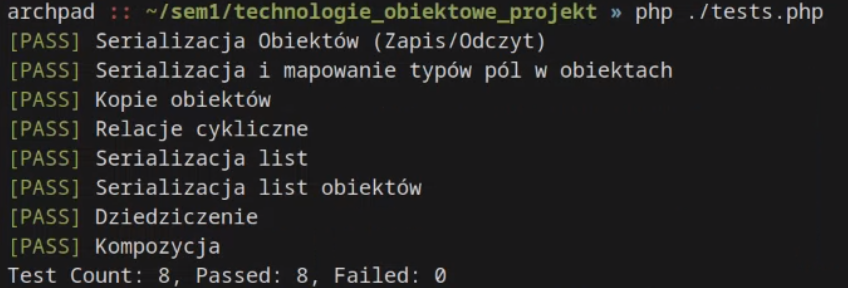
\includegraphics[width=0.9\textwidth]{materiały/raport}
	\caption{Raport wykonanych testów}
\end{figure}

\subsection{Test serializacji obiektów}
Jest to najbardziej podstawowy test, mają5cy na celu weryfikację działania mappera pod kątem zapisu i odczytu prostych obiektów, niezawierających list ani referencji do innych obiektów.

\begin{figure}[ht]
	\centering
	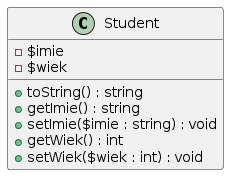
\includegraphics[width=0.3\textwidth]{materiały/student}
	\caption{Serializowana klasa \textbf{student}}
\end{figure}


\begin{empty}
	\begin{minted}[
		startinline,
		linenos,
		frame=lines,
		framesep=2mm,
		baselinestretch=1.2,
		fontsize=\footnotesize,
		breaklines,
		obeytabs=true,
		tabsize=2,
		]{text}
imie; wiek; id#
Tomek; 18; 666613345af2d
	\end{minted}
	\vspace{-10pt}
	\captionof{listing}{Wygenerowany plik TestSerializacjiObiektow-Student.csv}
\end{empty}


\begin{empty}
	\begin{minted}[
		startinline,
		linenos,
		frame=lines,
		framesep=2mm,
		baselinestretch=1.2,
		fontsize=\footnotesize,
		breaklines,
		obeytabs=true,
		tabsize=2,
		]{php}
public function test ()
{
	if ($this->mapper == null) {
		return $this->fail();
	}
	
	$student = new Student();
	$student->setWiek(18);
	$student->setImie("Tomek");
	
	$this->mapper->save($student);
	$fromFile = $this->mapper->read("./TestSerializacjiObiektow\Student.csv", Student::class);
	
	if (get_class($fromFile) != Student::class) {
		return $this->fail();
	}
	
	if ($student->toString() != $fromFile->toString()) {
		return $this->fail();
	}
	
	return $this->pass();
}
	\end{minted}
	\vspace{-10pt}
	\captionof{listing}{Logika testu.}
\end{empty}

\subsection{Test serializacji typów}
Kolejny, również prosty test, mający na celu sprawdzenie poprawności serializacji typów pól. Po zapisie sprawdzane jest, czy typy pól odczytanego obiektu zgadzają się z typami oryginalnego obiektu. 

\begin{empty}
	\begin{minted}[
		startinline,
		linenos,
		frame=lines,
		framesep=2mm,
		baselinestretch=1.2,
		fontsize=\footnotesize,
		breaklines,
		obeytabs=true,
		tabsize=2,
		]{php}
if (gettype($fromFile->getWysokosc()) != gettype($student->getWysokosc())) {
	return $this->fail();
}
if (gettype($fromFile->getWiek()) != gettype($student->getWiek())) {
	return $this->fail();
}
if (gettype($fromFile->getImie()) != gettype($student->getImie())) {
	return $this->fail();
}
	\end{minted}
	\vspace{-10pt}
	\captionof{listing}{Logika testu.}
\end{empty}

\subsection{Test kopii obiektów}
Test ma na celu zweryfikować, poprawność serializacji wielu referencji do tego samego obiektu, w obiekcie \textbf{A}, pola \mintinline{php}|$b1|  oraz \mintinline{php}|$b2| zawierają referencje do tego samego obiektu. Natomiast pole \mintinline{php}|$b3| zawiera referencje do innego obiektu tej samej klasy. Test upewnia się, że zostaną zserializowane tylko dwie instancje klasy \textbf{B}, oraz to, że zostaną one poprawnie zmapowane po odczytaniu.  

\begin{figure}[ht]
	\centering
	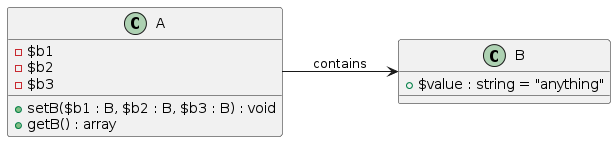
\includegraphics[width=0.75\textwidth]{materiały/kopie}
	\caption{Serializowane klasy}
\end{figure}

\begin{empty}
	\begin{minted}[
		startinline,
		linenos,
		frame=lines,
		framesep=2mm,
		baselinestretch=1.2,
		fontsize=\footnotesize,
		breaklines,
		obeytabs=true,
		tabsize=2,
		]{text}
b1@TestObjectCopies\B; b2@TestObjectCopies\B; b3@TestObjectCopies\B; id#
666619324645f; 666619324645f; 6666193246466; 6666193246459
	\end{minted}
	\vspace{-10pt}
	\captionof{listing}{Plik TestObjectCopies-A.csv}
\end{empty}


\begin{empty}
	\begin{minted}[
		startinline,
		linenos,
		frame=lines,
		framesep=2mm,
		baselinestretch=1.2,
		fontsize=\footnotesize,
		breaklines,
		obeytabs=true,
		tabsize=2,
		]{text}
value; id#
anything; 666619324645f
anything; 6666193246466
	\end{minted}
	\vspace{-10pt}
	\captionof{listing}{Plik TestObjectCopies-B.csv}
\end{empty}

\subsection{Test serializacji list}
Prosty test serializacji list typów prymitywnych. 

\begin{figure}[ht]
	\centering
	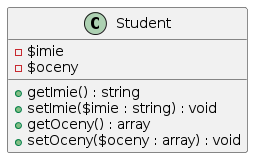
\includegraphics[width=0.35\textwidth]{materiały/sam_student}
	\caption{Mapowana klasa}
\end{figure}

\begin{empty}
	\begin{minted}[
		startinline,
		linenos,
		frame=lines,
		framesep=2mm,
		baselinestretch=1.2,
		fontsize=\footnotesize,
		breaklines,
		obeytabs=true,
		tabsize=2,
		]{text}
imie; ~oceny; id#
Szymek; 2,2,3,1; 66661932466e6
	\end{minted}
	\vspace{-10pt}
	\captionof{listing}{Plik TestLists-Student.csv}
\end{empty}

\subsection{Test serializacji list obiektów}
Jest to rozszerzenie poprzedniego testu o referencje do obiektów innej klasy. Idea testu pozostaje taka sama.

\begin{figure}[ht]
	\centering
	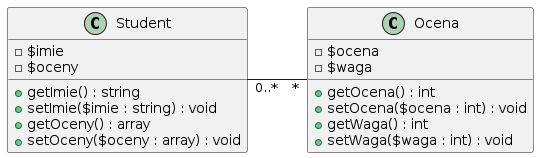
\includegraphics[width=0.7\textwidth]{materiały/st-oc}
	\caption{Mapowana klasa}
\end{figure}

Struktura plików .csv została zaprezentowana we wstępie. 


\subsection{Test - dziedziczenie}
W programowaniu obiektowym jednym z podstawowych narzędzie jest dziedziczenie oraz implementowanie. Oczywistym jest, że nasz mapper musi współpracować z obiektami posługującymi się tymi narzędziami. Test ten ma na celu weryfikację, czy odtworzony obiekt odpowiednio dziedziczy po klasie \mintinline{php}|Osoba| oraz czy implementuje interfejs \mintinline{php}|Witalny|.

\begin{figure}[ht]
	\centering
	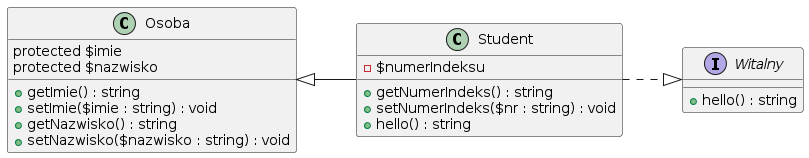
\includegraphics[width=0.82\textwidth]{materiały/dziedziczenie}
	\caption{Mapowana klasa}
\end{figure}

\begin{empty}
	\begin{minted}[
		startinline,
		linenos,
		frame=lines,
		framesep=2mm,
		baselinestretch=1.2,
		fontsize=\footnotesize,
		breaklines,
		obeytabs=true,
		tabsize=2,
		]{php}
if (!($fromFile instanceof Student)) {
	return $this->fail();
}

if (!($fromFile instanceof Osoba)) {
	return $this->fail();
}

if (!($fromFile instanceof Witalny)) {
	return $this->fail();
}
	\end{minted}
	\vspace{-10pt}
	\captionof{listing}{Logika testu}
\end{empty}

\begin{empty}
	\begin{minted}[
		startinline,
		linenos,
		frame=lines,
		framesep=2mm,
		baselinestretch=1.2,
		fontsize=\footnotesize,
		breaklines,
		obeytabs=true,
		tabsize=2,
		]{text}
		numerIndeksu; imie; nazwisko; id#
		abc123; Kamil; Ślimak; 6666193246903
	\end{minted}
	\vspace{-10pt}
	\captionof{listing}{Plik TestDziedziczenia-Student.csv}
\end{empty}


\subsection{Test - kompozycja}
Kolejnym narzędziem wykorzystywanym w technologiach obiektowych jest kompozycja. Poniższy test, zapewnia, pełną obsługę kompozycji przez naszego mappera. 

\begin{figure}[ht]
	\centering
	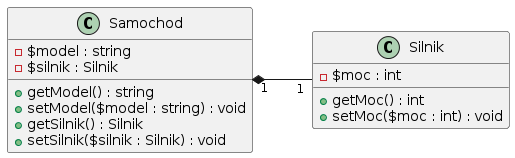
\includegraphics[width=0.7\textwidth]{materiały/kompozycja2}
	\caption{Mapowana klasa}
\end{figure}

\begin{empty}
	\begin{minted}[
		startinline,
		linenos,
		frame=lines,
		framesep=2mm,
		baselinestretch=1.2,
		fontsize=\footnotesize,
		breaklines,
		obeytabs=true,
		tabsize=2,
		]{php}
if ($fromFile->getModel() != $bmw->getModel()) {
	return $this->fail();
}

if (!($fromFile->getSilnik() instanceof Silnik)) {
	return $this->fail();
}

if ($fromFile->getSilnik()->getMoc() != $silnik->getMoc()) {
	return $this->fail();
}
	\end{minted}
	\vspace{-10pt}
	\captionof{listing}{Logika testu}
\end{empty}

\begin{empty}
	\begin{minted}[
		startinline,
		linenos,
		frame=lines,
		framesep=2mm,
		baselinestretch=1.2,
		fontsize=\footnotesize,
		breaklines,
		obeytabs=true,
		tabsize=2,
		]{text}
model; silnik@TestKompozycja\Silnik; id#
528i; 66661932469af; 66661932469a8
	\end{minted}
	\vspace{-10pt}
	\captionof{listing}{Plik TestKompozycja-Samochod.csv}
\end{empty}

\begin{empty}
	\begin{minted}[
		startinline,
		linenos,
		frame=lines,
		framesep=2mm,
		baselinestretch=1.2,
		fontsize=\footnotesize,
		breaklines,
		obeytabs=true,
		tabsize=2,
		]{text}
moc; id#
245KM; 66661932469af
	\end{minted}
	\vspace{-10pt}
	\captionof{listing}{Plik TestKompozycja-Silnik.csv}
\end{empty}

\subsection{Test relacji cyklicznych}
Relacje cykliczne zwane również rekurencyjnymi są ciekawym zjawiskiem, do których często dochodzi przez przypadek w środowiskach produkcyjnych. Niezależnie od tego, czy są dobrymi praktykami, czy nie, nasz mapper musi je wspierać. Ważne jest aby w trakcie odtwarzania obiektów, nie dopuścić do zapętlenia mappera. Takie zjawisko można wykryć przy pomocy tego testu. 

\begin{figure}[ht]
	\centering
	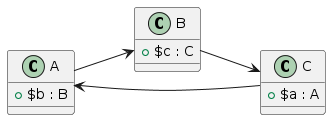
\includegraphics[width=0.5\textwidth]{materiały/relacje}
	\caption{Mapowana klasa}
\end{figure}

\begin{empty}
	\begin{minted}[
		startinline,
		linenos,
		frame=lines,
		framesep=2mm,
		baselinestretch=1.2,
		fontsize=\footnotesize,
		breaklines,
		obeytabs=true,
		tabsize=2,
		]{php}
if ($fromFile->b->c->a !== $fromFile) {
	return $this->fail();
}
	\end{minted}
	\vspace{-10pt}
	\captionof{listing}{Logika testu}
\end{empty}
